\documentclass[11pt,english]{article}

\setlength\parindent{0pt}
\usepackage{amssymb,amsmath,amscd,graphicx,fontenc,bbold,bm,amsthm,mathrsfs,mathtools}
\usepackage[pdftex,bookmarks,colorlinks,breaklinks]{hyperref} 
\usepackage{comment}
\hypersetup{linkcolor=blue,citecolor=red,filecolor=dullmagenta,urlcolor=blue}

\DeclarePairedDelimiter\abs{\lvert}{\rvert}%
\DeclarePairedDelimiter\norm{\lVert}{\rVert}%
\newcommand{\snxk}{\pi(x,k)}
\newcommand{\bnxk}{{\mathrm{N}}(x,k)}
\newcommand{\px}[1]{\pi(x,{#1})}
\newcommand{\Px}[1]{\Pi(x,{#1})}
\newcommand{\tr}{\mathrm{Trace}}
\newcommand{\real}{\mathbb{R}}
\newcommand{\pd}[1]{\frac{\partial}{\partial {#1}}}

\usepackage[top=3cm,bottom=3cm,right=2.3cm,left=2.3cm,twoside=false]{geometry}

\title{IFT6390-fundamentals of machine learning\\Assignment 2}
\author{Jonathan Guymont, Marzieh Mehdizadeh}

\date{}

\begin{document}

    \maketitle

    \section{Linear and non-linear regularized regression}

    \subsection{Linear Regression}

    (1) The set of parameters is $\theta=\{w_1,...,w_d, b\}$ where $w_i\in\real$ for $i=1,...,d$ and $b\in\real$. The $w_i$ are the coefficients of the different features of the inputs random variable $x_1,...,x_d$ and $b$ is the bias.\\

    (2) 
    \begin{equation}
        \begin{split}
            \hat{R}((x, t), f) 
            =& \sum_{i=1}^n (f(\bm{x}^{(i)})-t^{(i)})^2 \\
            =& \sum_{i=1}^n (b + \bm{w}^\top\bm{x}^{(i)}-t^{(i)})^2
        \end{split}
    \end{equation} 

    (3) We rewrite the loss with matrix instead. Let $X\in\real^{n\times d+1}$ be the design matrix where the rows are the different training examples and the first column is a row of ones that we add for convenience. Also lets redefine the weight vector as $\bm{w}^top=(b, w_1,...,w_d)$. In this new formulation of the input and parameters, we have that $\bm{w}^\top\bm{x}\equiv b + \bm{w}{'^top}\bm{x}'$, where "$'$" indicates the previous format. Let $\hat{Y}\in\real^n$ be the vector of preditions for all the training examples and $Y=(t^{(1)},....,t^{(n)})^\top$. We have $\hat{Y}\in\real^n=X\bm{w}$. It follows that $\hat{R}((x, t), f)=(\hat{Y}-Y)^\top(\hat{Y}-Y)=(X\bm{w}-Y)^\top(X\bm{w}-Y)^\top$

    \begin{equation}
        \begin{split}
            (X\bm{w}-Y)(X\bm{w}-Y)^\top 
            =& (-Y^\top + \bm{w}^\top X^\top)(X\bm{w}-Y) \\  
            =& \bm{w}^\top X^\top X\bm{w} - Y^\top X\bm{w} - \bm{w}^\top X^\top Y  + Y^\top Y  \\
            =& \bm{w}^\top X^\top X\bm{w} - 2\bm{w}^\top X^\top Y  + Y^\top Y~~~~(Y^\top X\bm{w}=\bm{w}^\top X^\top Y)  \\
        \end{split}
    \end{equation}

    where the last equality is true because $Y^\top X\bm{w}$ and $\bm{w}^\top X^\top Y$ are both the same scalar. And the derivative wrt $w$ is given by

    \begin{equation}
        \begin{split}
            \pd{\bm{w}} \bm{w}^\top X^\top X\bm{w} - 2\bm{w}^\top X^\top Y  + Y^\top Y
            =& 2X^\top X\bm{w} - 2 X^\top Y 
        \end{split}
    \end{equation}

    Setting the derivatives to zero
    \begin{equation}
        \begin{split}
            2X^\top X\bm{w} - 2 X^\top Y =& 0 \\
            X^\top X\bm{w}  =& X^\top Y \\
            \bm{w}*  =& (X^\top X)^{-1} X^\top Y \\
        \end{split}
    \end{equation}

    (4) While $||w||>\epsilon$ Do:
    $$
        \bm{w}_t = \bm{w}_{t-1} - \lambda \cdot 2(X^\top X\bm{w}_{t-1} - X^\top Y)
    $$
    where $\epsilon$ is some level of tolerence beyond which we are satisfied with the solution (gradient is flat enough).\\

    (5) The gradient can be rewriten as $2\cdot (X^\top \hat{Y} - X^\top Y)=2X^\top\cdot (\hat{Y} - Y)=2X^\top \bm{\varepsilon}$, where $\bm{\varepsilon}$ is the vector of errors (one for each examples). For a single point, the gradient is equal to $2\bm{x}^{(i)}\varepsilon^{(i)}$. We can see that the higher the error, the bigger the step. Also we always move in either the direction of $\bm{x}$ or in the opposite direction, and proportionnaly to the magnitude of the error.
    
    \subsection{Ridge Regression}

    (1) The gradient of the regulaized risk is equal to the gradient of the unregularized rist plus the gradient of the regularizer.
    \[
        \pd{\bm{w}} \hat{R} = 2(X^\top X\bm{w}_{t-1} - X^\top Y) + 2 \lambda \bm{w}
    \]

    (2) While $||w||>\epsilon$ Do:

       $$ \bm{w}_t \leftarrow \bm{w}_{t-1} - \eta \cdot 2(X^\top X\bm{w}_{t-1} - X^\top Y + \lambda \bm{w}_{t-1})
    $$
    where $\epsilon$ is some level of tolerance beyond which we are satisfied with the solution (the gradient is flat enough).\\

    (3) The gradient in (1) is already written in term of matrices. The regularized risk is given by
    $$
        \hat{R} = (X\bm{w}-Y)(X\bm{w}-\bm{t})^\top + \lambda ||\bm{w}||^2
    $$
    
    (4) Setting the derivative in (1) to zero
        
    \begin{equation}
        \begin{split}
            2(X^\top X\bm{w} - X^\top Y) + 2 \lambda \bm{w} =& 0 \\
            X^\top X\bm{w} + \lambda \bm{w} =& X^\top Y \\
            (X^\top X+ \lambda I) \bm{w} =& X^\top Y \\
             \bm{w}* =& (X^\top X+ \lambda I)^{-1}X^\top Y \\
        \end{split}
    \end{equation}

    If $\lambda=0$ whatever $N$ is, the empirical risk will equal to the unregularized one. The number of examples $N$ do not affect the shape of the gradient (the gradient is always in $\real^d$ whatever $N$ is).

    \subsection{Regression with a fixed non-linear pre-processing}

    (1) $\tilde{f}_k (x)=b + \sum_{i=1}^k w_i x^i = b + \bm{w}^\top \phi_k(x)$\\

    (2) $b$ is a scalar and $w_1,...,w_k$ are also scalars and the coefficient of the polynomial terms. Therefore dimension $d=1$ we will have $k+1$ parameters\\
    
    (3) $\phi_1(x)=x$ so this one is a linear regression. \\

    $\tilde{f}_1 (\bm{x})=b + w_1 x_1 + w_2 x_2$\\

    $\tilde{f}_2 (\bm{x})=b + w_1 x_1 + w_2 x_2 + w_3 x_1^2 + w_4 x_2^2 + w_5 x_1 x_2$\\

    $\tilde{f}_3 (\bm{x})=b + w_1 x_1 + w_2 x_2 + w_3 x_1^2 + w_4 x_2^2 + w_5 x_1 x_2 + w_6 x_1^2x_2 + w_7 x_1x_2^2 + w_8x_1^3 + w_9x_2^3$

    (4) For each powers $1,2,...,k$ we need $d$ coefficients, i.e. $dk$ parameters. We also need coefficient for the different combination of inputs (eg $x_1x_2$). IF $p$ is the degree of polynomial up to $k$, then one can prove the complexity by induction which it equal to:
    
    $$\sum_{p=1}^{k} \binom{d-1+p}{p}.$$



	\section{Practical Part}
	
	\textbf{Comment question 6}: Figure 3 show the predictions of 3 polynomial regression of different degrees fitted using gradient descent. We can see that models with higher degrees seems to fit the training observations better. We can also see that it is quite the opposite when we compare the models to the ground truth $h(x)$. Table 1 show the mean square errors of the fitted models computed on both the training set and the validation set. We can see that while the loss on the training set is lower for higher degree, it is the opposite for looses computed on the test set. This was expected since the ground truth is a polynomial of degree one. Thus the models with $l>1$ have to much capacity, which is particularly problematic given the very small training set, since in order to not overfit, the models would have to learn that $w_k=0$ for $k>1$. 
	
	\begin{table}[h!]
		\centering
		
		\begin{tabular}{c|cc}
			$l$ & train & test \\ 
			\hline 
			1 & 0.5654 & 0.5783  \\ 
			2 & 0.5549  & 0.6295 \\ 
			5 & 0.2722 & 0.771  \\ 
		\end{tabular}
		
		\caption{Mean square error of the fitted polynomial regressions of degree $l$. The MSE it reported for both the training and the test set} 
		
	\end{table}
	
	\begin{figure}[h!]
		\centering
		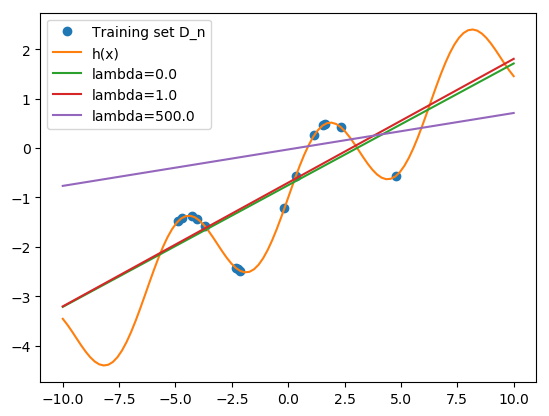
\includegraphics{../question3and4}
		\caption[Question 3 and 4]{Fitted ridge regression with different regularization constant}
		\label{fig:question3and4}
	\end{figure}
	
	\begin{figure}[h!]
		\centering
		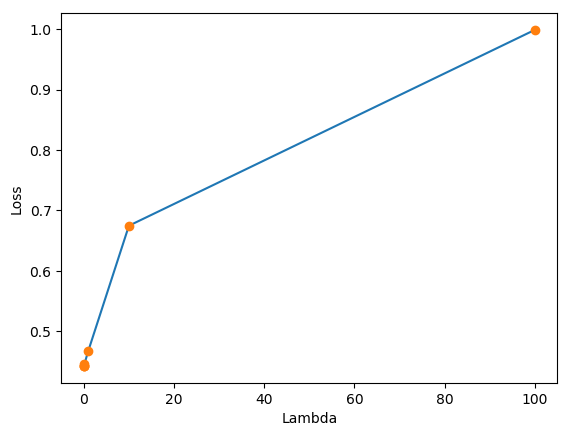
\includegraphics{../question5}
		\caption[Question 5]{Effect of the regularization constant $\lambda$ on the MSE loss of a simple linear regression}
		\label{fig:question5}
	\end{figure}
		
	\begin{figure}[h!]
		\centering
		\includegraphics{../question6}
		\caption[Question 6]{Fitted ridge regression with polynomial degrees}
		\label{fig:question6}
	\end{figure}

\end{document}